\documentclass[11pt]{article}

\usepackage{graphicx}
\usepackage{svg}
\usepackage{graphbox}
\usepackage{multicol}
\usepackage{amsmath}
\usepackage{amssymb}
\usepackage{mathtools}
\usepackage{pgfplots}
\usepackage{cancel}
\usepackage{xcolor,colortbl}
\usepackage[colorlinks=true, allcolors=blue]{hyperref}
\usepackage{float}

\usepackage{enumerate}

\oddsidemargin=-.3in
\evensidemargin=-.5in
\textwidth=7in
\topmargin=-1in
\textheight=9.7in

\parindent=.3in
\pagestyle{plain}

\definecolor{Gray}{gray}{0.9}
\definecolor{Yellow}{rgb}{255,255,0}
\newcolumntype{y}{>{\columncolor{Yellow}}c}

\allowdisplaybreaks

\newenvironment{problems}


\begin{document}



\begin{centering}
{\huge \bf Exercise 2} \smallskip

{\Large \em Pattern Recognition, Fall 2021

Nico Aebischer

Max Jappert

}
\end{centering}

\begin{enumerate}[1.]
	\item The error rates for the three images can be seen in the output of our program, which is listed on this page. Thereafter the three outputted images are shown.
	
	\begin{verbatim}
##########-##########-##########
TRAINING DATA
(128000,)
(128000,)
----- ----- -----
Total Error WITHOUT Prior = 4894
false positive rate = 0.02415625
false negative rate = 0.014078125
----- ----- -----
Total Error WITH Prior = 4303
false positive rate = 0.0160546875
false negative rate = 0.0175625
----- ----- -----
TEST DATA PORTRAIT
(166400,)
(166400,)
----- ----- -----
Total Error WITHOUT Prior = 18044
false positive rate = 0.10468149038461538
false negative rate = 0.0037560096153846155
----- ----- -----
Total Error WITH Prior = 22715
false positive rate = 0.1323016826923077
false negative rate = 0.004206730769230769
----- ----- -----
TEST DATA FAMILY
(540000,)
(540000,)
----- ----- -----
Total Error WITHOUT Prior = 35481
false positive rate = 0.004629629629629629
false negative rate = 0.06107592592592593
----- ----- -----
Total Error WITH Prior = 43539
false positive rate = 0.003174074074074074
false negative rate = 0.0774537037037037
----- ----- -----
##########-##########-##########

	\end{verbatim}
	
	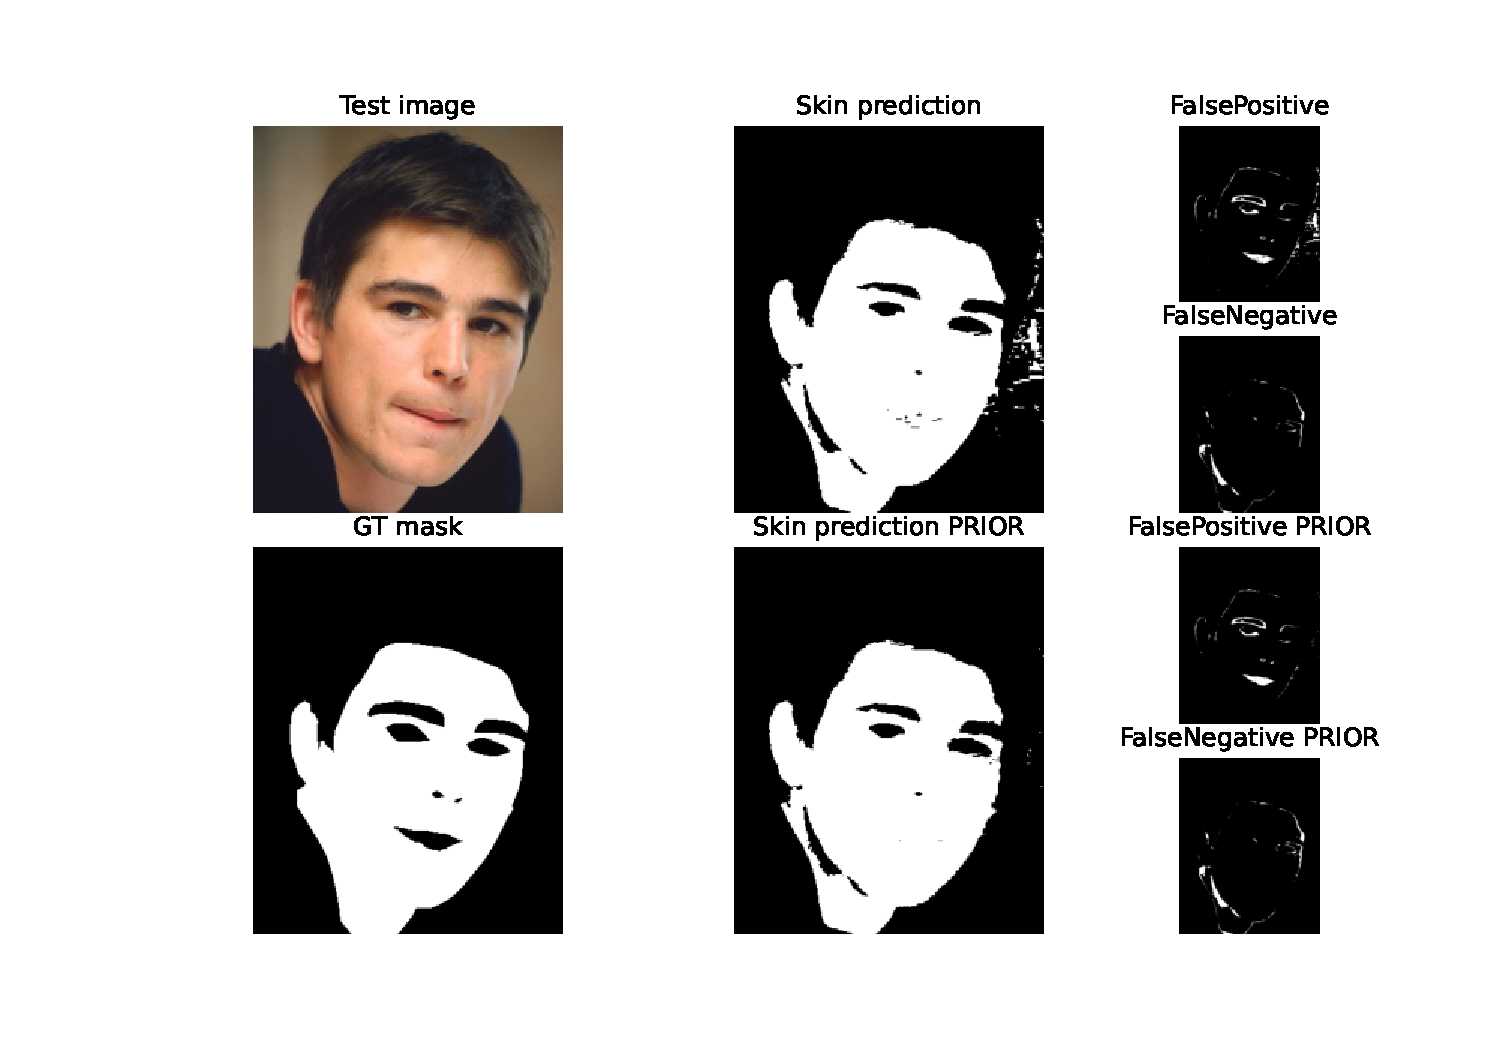
\includegraphics[width=6in]{Training-MVND.pdf}\\
	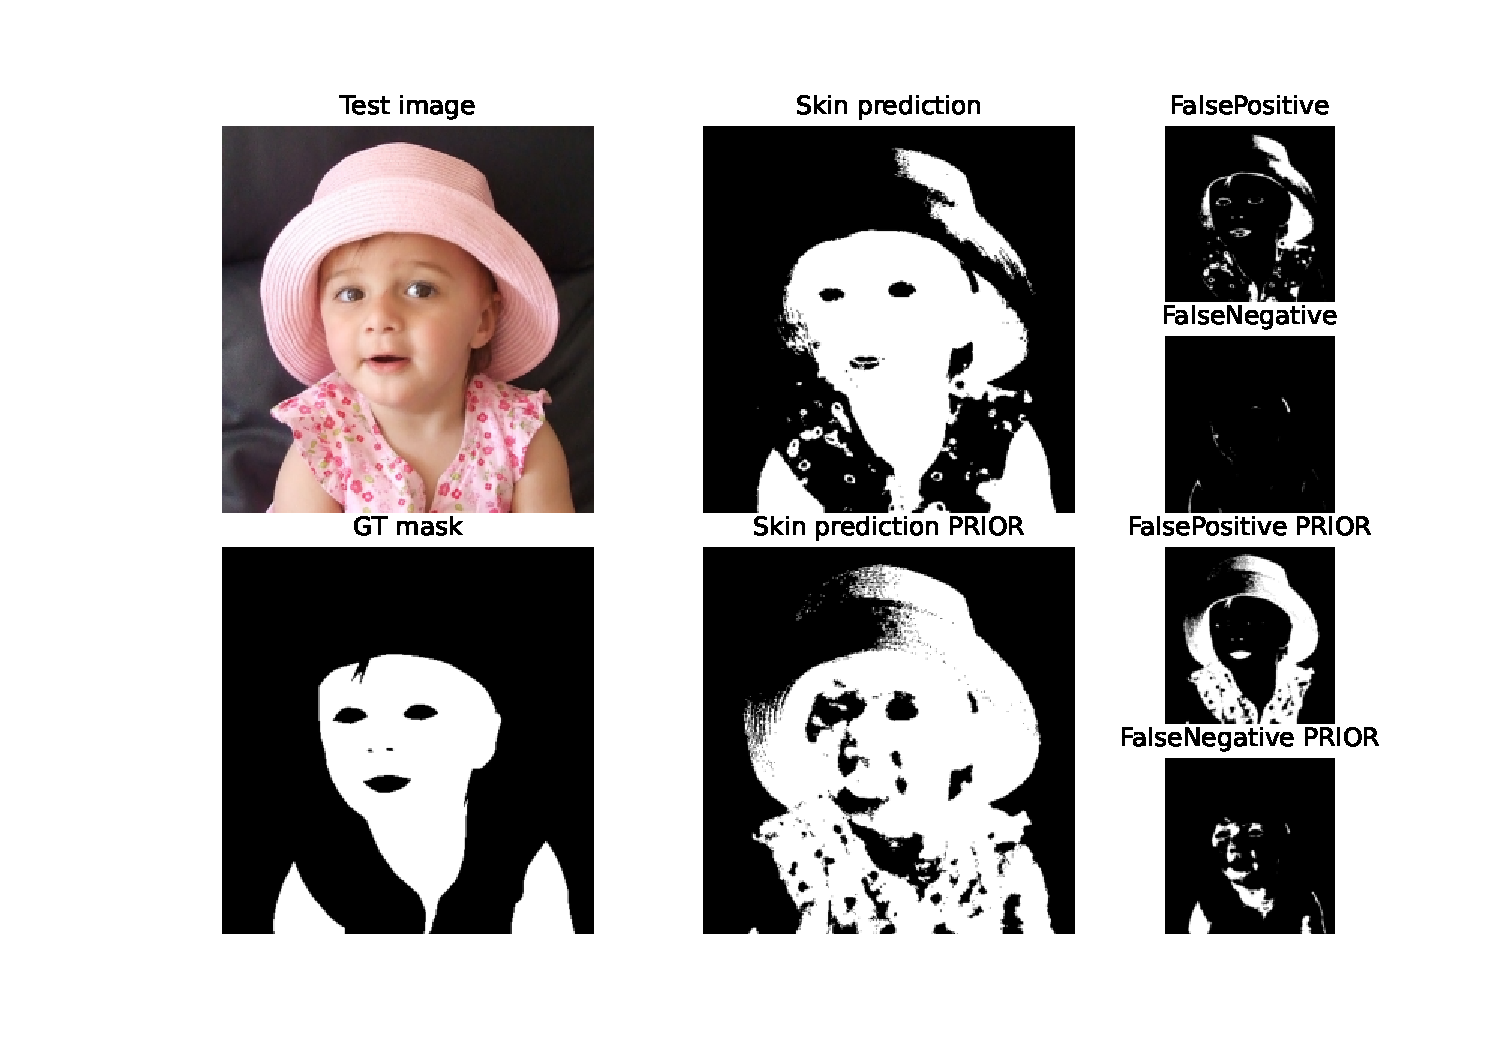
\includegraphics[width=6in]{Test-portrait-MVND.pdf}\\
	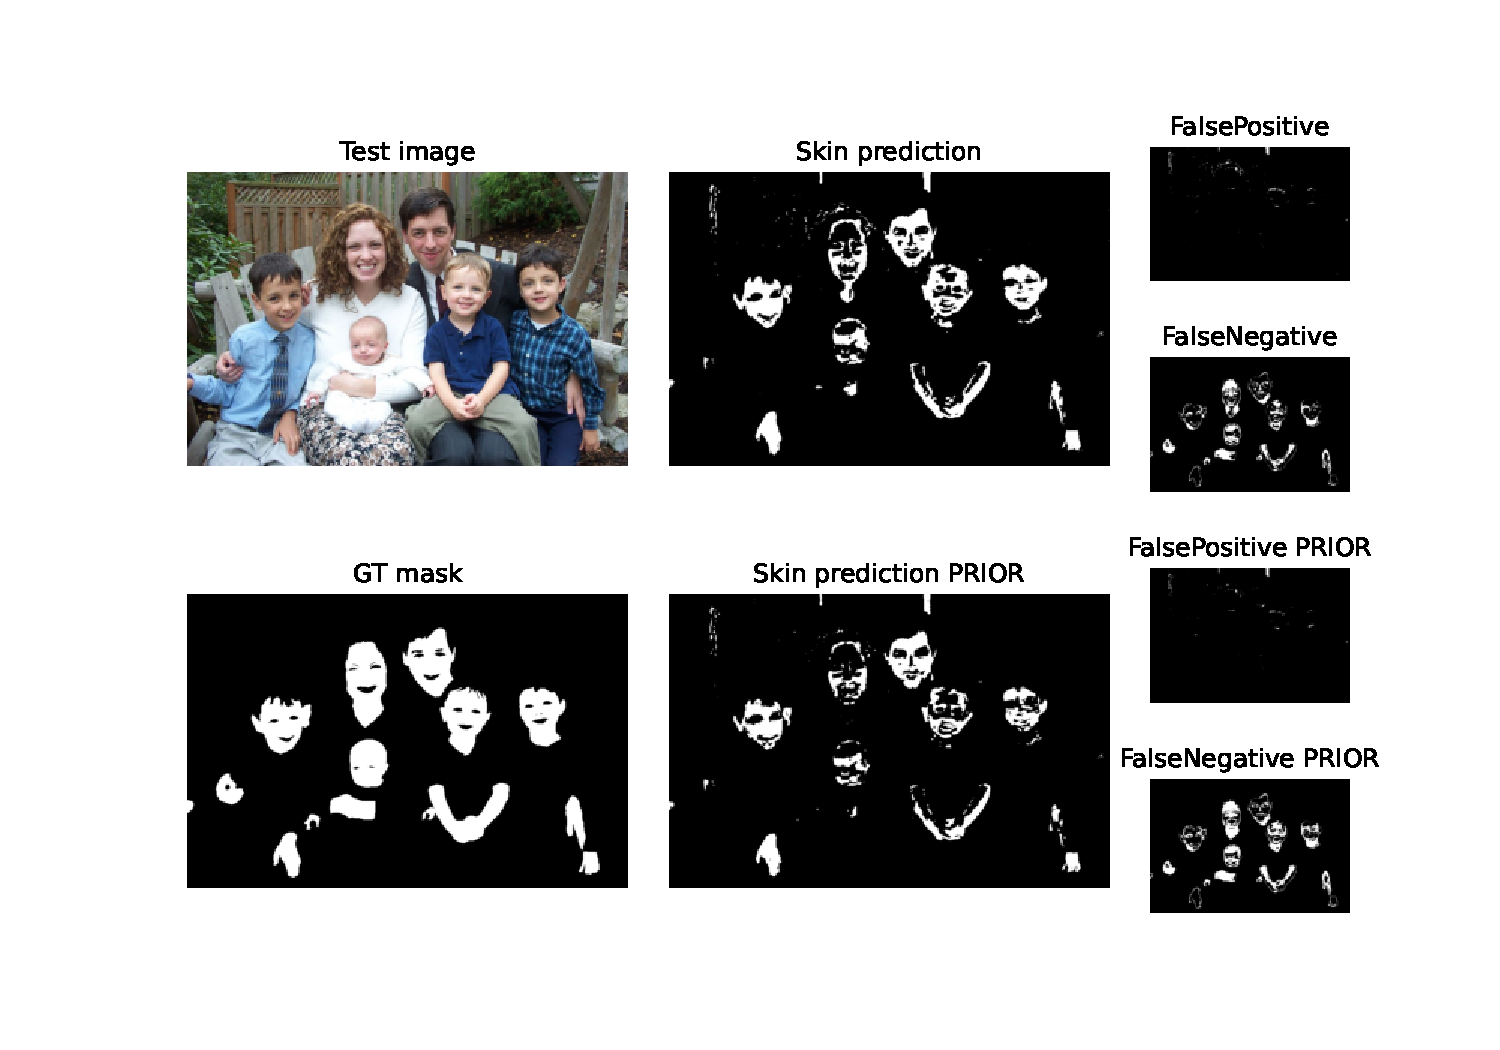
\includegraphics[width=6in]{Test-family-MVND.pdf}

	\item Skin prior: 0.3699921875\\Non-skin prior: 0.6300078124999999
	\item The prior represents the probability of a sample (in this case a pixel) belonging to a class without taking any evidence into account (in this case without considering the actual image). Therefore we calculated the priors by calculating the the proportion of the training mask which is classified as skin or non-skin for the training image. Thereby the priors represent the naive probability of a pixel belonging to each class, without considering the actual pixel to be classified. 
	\item While including the prior into the calculation improves the classification performance on the training image, the classification is less accurate with the prior included for both images the algorithm hasn't seen yet. This is because the prior has overfitted the training data. The proportion of skin in an image is not correlated to how skin can be classified generally while that proportion is very closely correlated to the image which was used for calculating this value.
	\item 
\end{enumerate}




\end{document}